\documentclass[12pt, a4paper]{article}

% Пакети за српски ћирилични текст
\usepackage[T2A]{fontenc}
\usepackage[utf8]{inputenc}
\usepackage[serbianc]{babel}

% Остали корисни пакети
\usepackage{amsmath}
\usepackage{amssymb}
\usepackage{amsthm}
\usepackage{geometry}
\usepackage{hyperref}
\usepackage{graphicx}
\usepackage{float}
\usepackage{listings}
\usepackage{xcolor}

% TLA+ стил за listings
\lstdefinelanguage{tla}{
    morekeywords={MODULE, EXTENDS, VARIABLES, CONSTANTS, ASSUME,
                  INSTANCE, LOCAL, RECURSIVE,
                  IF, THEN, ELSE, CASE, OTHER,
                  LET, IN,
                  TRUE, FALSE, BOOLEAN, STRING,
                  SUBSET, UNION, DOMAIN, ENABLED, UNCHANGED,
                  Init, Next, Spec},
    sensitive=true,
    morecomment=[l]{\*},
    morecomment=[s]{(*}{*)},
    morestring=[b]",
}

\lstset{
    language=tla,
    basicstyle=\ttfamily\small,
    keywordstyle=\bfseries\color{blue!70!black},
    commentstyle=\itshape\color{gray},
    stringstyle=\color{green!50!black},
    frame=single,
    backgroundcolor=\color{gray!8},
    rulecolor=\color{gray!40},
    numbers=left,
    numberstyle=\tiny\color{gray},
    numbersep=6pt,
    breaklines=true,
    keepspaces=true,
    showstringspaces=false,
}

% Подешавање маргина
\geometry{
    left=2.5cm,
    right=2.5cm,
    top=2.5cm,
    bottom=2.5cm
}

% Дефиниција теорема, лема, итд.
\theoremstyle{plain}
\newtheorem{teorema}{Теорема}[section]
\newtheorem{lema}[teorema]{Лема}
\newtheorem{posledica}[teorema]{Последица}

\theoremstyle{definition}
\newtheorem{definicija}[teorema]{Дефиниција}
\newtheorem{primer}[teorema]{Пример}

\theoremstyle{remark}
\newtheorem*{napomena}{Напомена}

% Наслов документа
\title{\textbf{Формалне методе} \\ (Увод у TLA+)}
\author{Филип Марић \\ Александар Ивановић}
\date{\today}

% -------------------------------------------------------
\begin{document}

\maketitle
\newpage
\tableofcontents
\newpage
\section{Предговор}
\newpage

% -------------------------------------------------------
\section{Увод - Шта је TLA?}
TLA је језик који за писање и провервање спецификација или дизајнирање система.
Када имамо нашу спецификацију тада га можемо користити за
тестирање грешака у дизајну и пре него што почнемо са самом имплементацијом система.
Развијен је од стране Леслија Лампорта, који је такође осмислио језик \LaTeX  
што је скраћеница од Лампортов \TeX.
TLA је скраћеница за Temportal Logic of Actions.

\subsection{Инсталација}

Да бисмо почели да пишемо и проверавамо TLA+ спецификације, потребно је инсталирати следеће алате:

\begin{itemize}
    \item \textbf{Java} -- TLA+ алати захтевају Java Runtime Environment (JRE 8 или новији).
    Може се преузети са \url{https://www.java.com}.

    \item \textbf{TLA+ Toolbox} -- званични IDE за TLA+, доступан на
    \url{https://github.com/tlaplus/tlaplus/releases}.
    Садржи TLC model checker и TLAPS (TLA+ Proof System).

    \item \textbf{VS Code додатак (алтернатива)} -- за кориснике Visual Studio Code,
    постоји додатак \texttt{TLA+ by alygin} доступан у VS Code Marketplace-у.
\end{itemize}

\subsubsection{Кораци инсталације (TLA+ Toolbox)}

\begin{enumerate}
    \item Преузети инсталациони пакет са званичне странице за свој оперативни систем.
    \item Покренути инсталацију и пратити упутства.
    \item Покренути Toolbox и креирати нови пројекат: \textit{File > Open Spec > Add New Spec}.
    \item Написати прву спецификацију и покренути TLC model checker.
\end{enumerate}
\subsubsection{Кораци инсталације (VS Code едитор)}
Ми ћемо у овим материјалима користити VS Code едитор (надље само \textbf{вс едитор})
и објаснићемо примере и инсталацију на примеру њега у оперативном систему линукс. Напомињемо да се TLA+ Toolbox
више не одржава, али да се и даље може скинути и користити. Вс едитор је постао
стандард за писање спецификација и TLA се може користити кроз њега као додатак.
Иначе напомињемо да је вс едитор постао популаран едитор за разне програмске језике 
управо због модуларности коју пружа богат избор додатака.

Изаберемо иконицу са додацима где се они инсталирају као на слици 1.
\begin{figure}[H]
    \centering
    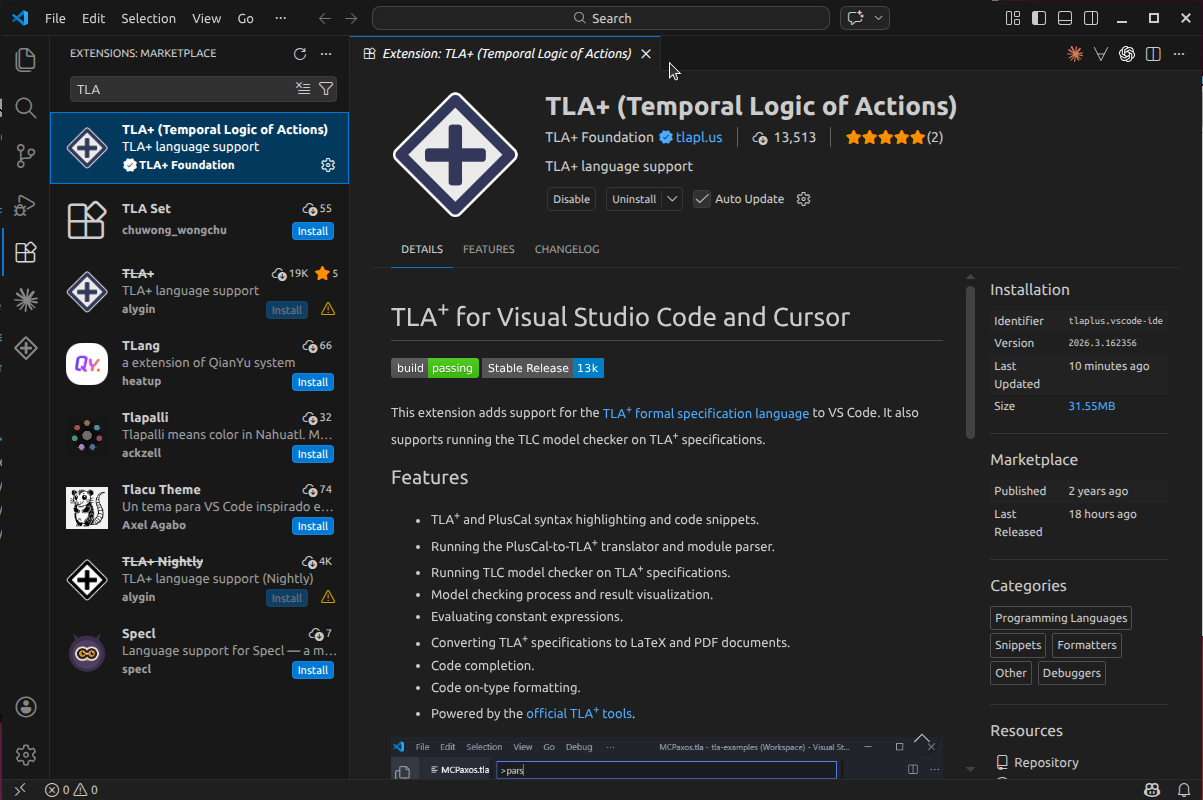
\includegraphics[width=0.7\textwidth]{Images/Instalacija.png}
    \caption{Инсталација TLA+ додатка у VS Code}
\end{figure}
Приликом избора додатка који ћемо инсталирати у претрагу укуцамо
TLA и одаберемо додак као на слици. На крају процеса едитор треба да 
изгледа као на слици 2.
\begin{figure}[H]
    \centering
    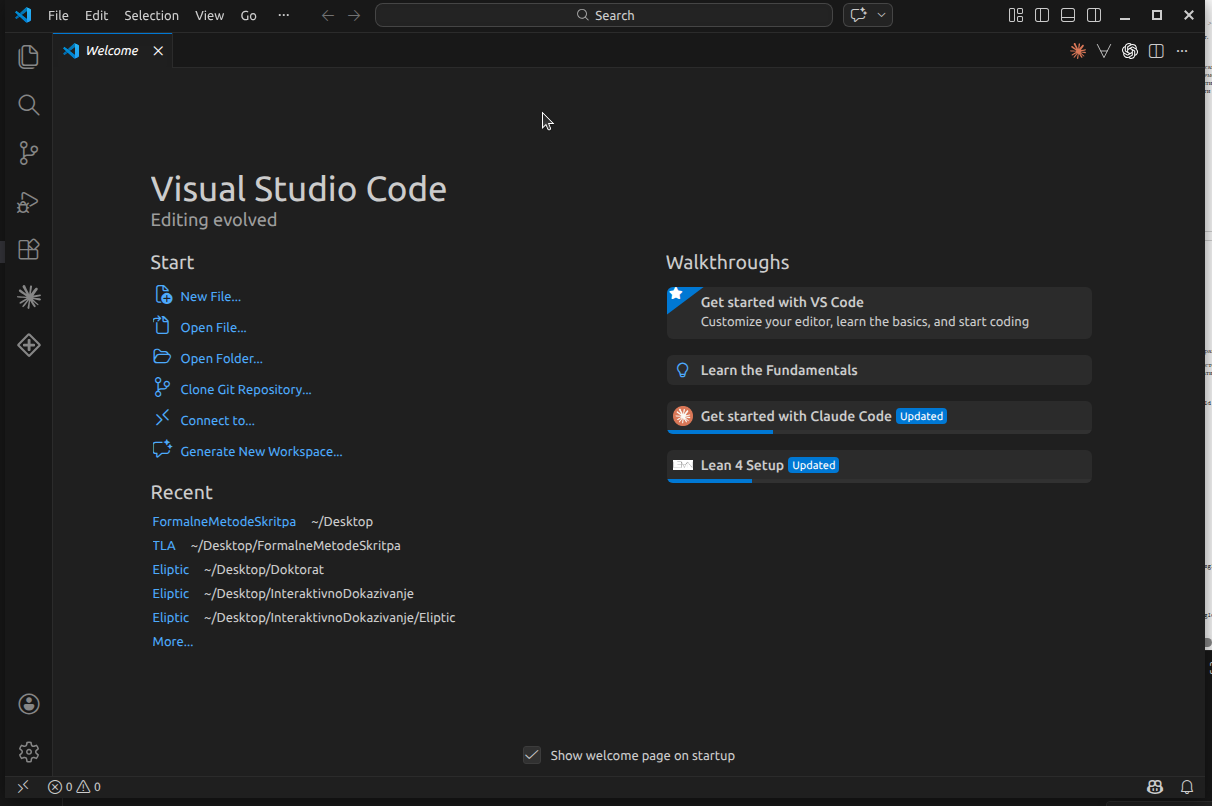
\includegraphics[width=0.7\textwidth]{Images/VSEditor.png}
    \caption{VS Code едитор са TLA+ додатком}
\end{figure}

Сада дајемо мали пример TLA спецификације како би тестирали дали окружење ради добро.

\begin{lstlisting}
---- MODULE Counter ----
EXTENDS Naturals

VARIABLES counter

Init == counter = 0

Increment == counter' = counter + 1

Next == Increment

Spec == Init /\ [][Next]_counter
====
\end{lstlisting}
У VS code едитору ћемо направити нов текстуални фајл са наставком \textbf{.tla}
\newpage
% -------------------------------------------------------
\section{Основни појмови}

\begin{definicija}
    Овде иде дефиниција неког појма.
\end{definicija}

\begin{primer}
    Овде иде пример.
\end{primer}

% -------------------------------------------------------
\section{Неки примери}
Овде дајемо неке примере из реалног живота и свакодневне програмерске праксе.
\begin{primer}[Outbox pattern]
Outbox pattern је техника којом се у истој трансакцији уписује промена у базу и порука у outbox табелу.
Засебан процес затим чита outbox и шаље поруке ка брокеру, па се порука чисти тек након потврде.

\textbf{TLA+ код (издвојени део спецификације):}
\begin{lstlisting}
VARIABLES db, outbox, broker, sent, acked, allMsgs, nextMsgId

CreateOrder(o) ==
    LET m == [id |-> nextMsgId, order |-> o] IN
    /\ db[o] = "NEW"
    /\ db' = [db EXCEPT ![o] = "CREATED"]
    /\ outbox' = outbox \cup {m}
    /\ allMsgs' = allMsgs \cup {m}
    /\ nextMsgId' = nextMsgId + 1
    /\ UNCHANGED <<broker, sent, acked>>

RelaySend(m) ==
    /\ m \in outbox
    /\ broker' = broker \cup {m}
    /\ sent' = sent \cup {m.id}
    /\ UNCHANGED <<db, outbox, acked, allMsgs, nextMsgId>>

AckFromBroker(m) ==
    /\ m \in broker
    /\ acked' = acked \cup {m.id}
    /\ UNCHANGED <<db, outbox, broker, sent, allMsgs, nextMsgId>>

CleanupOutbox(m) ==
    /\ m \in outbox
    /\ m.id \in acked
    /\ outbox' = outbox \ {m}
    /\ UNCHANGED <<db, broker, sent, acked, allMsgs, nextMsgId>>
\end{lstlisting}
\end{primer}

\begin{primer}[Outbox pattern]

\end{primer}

\begin{primer}[Outbox pattern]

\end{primer}

\begin{primer}[Outbox pattern]

\end{primer}



% \begin{teorema}
%     Овде стоји исказ теореме.
% \end{teorema}

% \begin{proof}
%     Овде иде доказ теореме.
% \end{proof}

% \begin{lema}
%     Овде стоји исказ леме.
% \end{lema}

% \begin{posledica}
%     Овде стоји последица.
% \end{posledica}

% % -------------------------------------------------------
% \section{Закључак}

% Овде иде закључак.

% -------------------------------------------------------
\newpage
\nocite{lamportLearningTLA,learnTLAIndex}
\bibliographystyle{plain}
\bibliography{literatura}

\end{document}
